\documentclass{report}
\usepackage[utf8]{inputenc}
\usepackage{enumitem}
\usepackage[a4paper]{geometry}
\usepackage{amsmath, amssymb}
\usepackage{setspace}
\usepackage{pifont}
\usepackage{xcolor}
\usepackage{graphicx}
\usepackage{hyperref} 
\usepackage{float}
\usepackage{booktabs}
\usepackage{geometry}
\geometry{a4paper, margin=1in}
\renewcommand{\arraystretch}{1.2} % Espaciado entre filas


\geometry{top=2cm, bottom=2.0cm, left=1cm, right=1cm}


\begin{document}

\noindent\textbf{\Large Estado de Arte Paper}\\
\textbf{Albert Montenegro}\\[0.1cm]

\small 
\setcounter{tocdepth}{1}
\tableofcontents

\chapter{XAI en Marcha}

\section{Estado del Arte en Explainable AI (XAI) para el Análisis de la Marcha}

El campo de la Inteligencia Artificial Explicable (XAI) ha demostrado ser fundamental para abordar la opacidad de los modelos de aprendizaje automático aplicados al análisis de la marcha. La capacidad de interpretar los resultados generados por estos modelos facilita su aceptación en contextos clínicos y permite identificar patrones biomecánicos relevantes para diagnósticos y tratamientos. A continuación, se presenta una revisión de los estudios más destacados en esta área.

\subsection{Explaining the Unique Nature of Individual Gait Patterns with Deep Learning}
Este trabajo, publicado por Horst et al. (2019) en \textit{Scientific Reports}, se enfoca en la interpretabilidad de los modelos de aprendizaje profundo aplicados a la marcha. Utilizando la técnica de \textit{Layer-wise Relevance Propagation} (LRP), los autores logran identificar regiones específicas del ciclo de marcha que contribuyen a la clasificación de patrones únicos de individuos. Este enfoque no solo mejora la comprensión de las predicciones, sino que también incrementa la confianza de los clínicos en el uso de redes neuronales convolucionales (CNN) para aplicaciones de rehabilitación y diagnóstico.

\subsection{Interpretability of Input Representations for Gait Classification in Patients after Total Hip Arthroplasty}
Dindorf et al. (2020), en \textit{Sensors}, investigan cómo distintas representaciones de entrada afectan la interpretabilidad de modelos de clasificación de marcha en pacientes con artroplastia total de cadera. Utilizando técnicas como \textit{Local Interpretable Model-Agnostic Explanations} (LIME), el estudio demuestra que las estadísticas descriptivas y las características automáticas generadas con \textit{tsfresh} son clave para identificar movimientos relevantes de cadera y rodilla. Los modelos SVM y MLP lograron desempeños sobresalientes, con precisiones superiores al 97\%.

\subsection{Explainable Machine Learning in Clinical Gait Analysis}
Slijepcevic et al. (2021), en \textit{ACM Transactions on Computing for Healthcare}, implementan \textit{Layer-wise Relevance Propagation} (LRP) para analizar patrones de marcha en pacientes con trastornos clínicos. Los modelos evaluados incluyen CNNs, MLPs y SVMs, mostrando que las regiones temporales clave en las fuerzas de reacción al suelo son fundamentales para las predicciones. Este estudio subraya la importancia de validar estadísticamente las explicaciones generadas y su relevancia clínica mediante \textit{Statistical Parametric Mapping} (SPM).

\subsection{Explainable Gait Recognition with Prototyping Encoder-Decoder}
Moon et al. (2022), en \textit{PLOS ONE}, introducen un modelo basado en un \textit{encoder-decoder} para el reconocimiento de marcha en entornos abiertos. Utilizando mapas de atribución generados por Grad-CAM, los autores identifican las señales más relevantes en modalidades como presión y aceleración. Este enfoque destaca por su robustez frente a variaciones en los datos y su capacidad para generalizar en escenarios biométricos y clínicos.

\subsection{Leveraging Explainable Machine Learning to Identify Gait Biomechanical Parameters Associated with ACL Injury}
Kokkotis et al. (2022), en \textit{Scientific Reports}, combinan técnicas de XAI con aprendizaje automático para identificar parámetros biomecánicos asociados a lesiones del ligamento cruzado anterior (ACL). Utilizando SHAP, el estudio demuestra que características como el ángulo de flexión de la rodilla y los momentos articulares de la cadera son esenciales para clasificar pacientes con y sin reconstrucción de ACL. Los modelos SVM y NN alcanzaron precisiones superiores al 92\%.

\subsection{Trustworthy Visual Analytics in Clinical Gait Analysis}
Rind et al. (2022), en un taller de la IEEE, desarrollan una herramienta interactiva (gaitXplorer) que combina Grad-CAM con visualizaciones interactivas para analizar patrones de marcha en pacientes con parálisis cerebral. Este enfoque permite a los clínicos interpretar resultados automáticos y comparar datos de pacientes con promedios grupales, incrementando la confianza en los modelos automáticos.

\subsection{XAI and Wearable Sensor-Based Gait Analysis to Identify Patients with Osteopenia and Sarcopenia in Daily Life}
Kim et al. (2022), en \textit{Biosensors}, utilizan XAI para analizar parámetros de marcha en mujeres mayores con osteopenia y sarcopenia. Los modelos ML (e.g., XGBoost, RF) superaron a los modelos DL (e.g., CNN, BiLSTM) en la clasificación, destacando la utilidad de parámetros estadísticos descriptivos. Técnicas como SHAP y Grad-CAM permiten interpretar los resultados y mejorar la confianza en los modelos.

\subsection{Explainable Machine Learning in Human Gait Analysis: A Study on Children With Cerebral Palsy}
Slijepcevic et al. (2023), en \textit{IEEE Access}, investigan patrones de marcha en niños con parálisis cerebral utilizando datos de análisis de marcha tridimensionales (3DGA). Los modelos evaluados incluyen CNNs, SNNs, RF y DT, destacando la importancia de las señales sagitales de tobillo y rodilla para la clasificación. Técnicas como Grad-CAM y la importancia de características permiten explicar las predicciones y orientar la evaluación clínica.

\subsection{Identification and Interpretation of Gait Analysis Features and Foot Conditions by Explainable AI}
Özateş et al. (2024), en \textit{Scientific Reports}, presentan un pipeline de ML para identificar condiciones específicas del pie a partir del análisis de marcha. Los modelos evaluados incluyen SVM, RF y KNN, combinados con técnicas XAI como LIME para identificar las características más relevantes. El estudio demuestra que la combinación de ML y XAI puede automatizar y mejorar la interpretación del análisis de marcha.

\subsection{A New Method Applied for Explaining the Landing Patterns}
Xu et al. (2024), en \textit{Heliyon}, proponen un modelo basado en LRP para explicar patrones de aterrizaje en movimientos biomecánicos. A través de \textit{Statistical Parametric Mapping} (SPM) y análisis del tamaño del efecto, se validan las explicaciones generadas por el modelo. Este enfoque destaca por identificar contribuciones relevantes en las señales de las articulaciones del tobillo y la rodilla, particularmente en el plano sagital.

\subsection{Conclusión}
Los estudios revisados destacan la aplicación de XAI en el análisis de la marcha, permitiendo interpretaciones detalladas y validadas estadísticamente de los modelos de aprendizaje automático. Técnicas como LRP, Grad-CAM y SHAP han demostrado ser fundamentales para mejorar la aceptación clínica y la confianza en los modelos automáticos. Este avance abre nuevas posibilidades para el diagnóstico, rehabilitación y planificación de tratamientos en biomecánica clínica.

\newpage



\begin{table}[ht]
    \footnotesize
    \centering
    \begin{tabular}{@{}p{1.5cm}p{2cm}p{1.5cm}p{3cm}p{2cm}p{2.5cm}p{1.5cm}p{2.5cm}}
    \toprule
    \textbf{Autores} & \textbf{Modelo} & \textbf{XAI} & \textbf{Tarea} & \textbf{Dispositivo} & \textbf{Entrada} & \textbf{Multiclase} & \textbf{Exactitud (\%)} \\
    \midrule
    Horst et al. (2019) & CNN & LRP & Patrones únicos de marcha individual & Plataforma de fuerza & GRF normalizadas & No & 99.4 \\
    Dindorf et al. (2020) & SVM, MLP & LIME & Clasificación tras artroplastia total de cadera & IMUs & Características automáticas y estadísticas & No & 97.3 \\
    Dindorf et al. (2021) & RF, SVM & SHAP & Interpretación de datos de postura espinal & IMUs & Ángulos funcionales & No & 95.0 \\
    Slijepcevic et al. (2021) & CNN, SVM & LRP & Análisis de marcha clínica en trastornos & GRF & Señales temporales clave & Sí & 92.0 / 85.0 \\
    Moon et al. (2022) & Autoencoder & Grad-CAM & Reconocimiento de marcha en open set & Plantillas con sensores & Presión, aceleración y rotación & No & 90.0 \\
    Kim et al. (2022) & XGBoost & SHAP & Identificación de osteopenia y sarcopenia & Sensores portables & Parámetros biomecánicos & No & 88.7 \\
    Rind et al. (2022) & CNN & Grad-CAM & Patrones de marcha en parálisis cerebral & 3DGA & Señales angulares y GRF & Sí & 87.0 / 75.0 \\
    Kokkotis et al. (2022) & SVM, NN & SHAP & Diagnóstico de lesión de ACL & Plataforma de fuerza & Ángulos y momentos articulares & Sí & 94.9 / 89.0 \\
    Slijepcevic et al. (2023) & RF, CNN & Grad-CAM & Patrones de marcha en niños con parálisis cerebral & 3DGA & Ángulos y GRF & Sí & 93.4 \\
    Xu et al. (2024) & ANN & LRP & Reconocimiento de patrones de aterrizaje & IMUs & Señales cinéticas y cinemáticas & No & 99.5 \\
    Özateş et al. (2024) & SVM, RF & LIME & Diagnóstico de condiciones del pie & IMUs & Ángulos funcionales & Sí & 87.0 \\
    \bottomrule
    \end{tabular}
    \caption{Resumen del estado del arte en Explainable AI (XAI) aplicado al análisis de la marcha.}
    \label{tab:state_of_art}
    \end{table}

    \subsection{Clasificación Multiclase}
    En el trabajo de \textbf{Rind et al. (2022)}, se realiza una tarea de clasificación multiclase. Este artículo aborda el análisis de patrones de marcha en pacientes con parálisis cerebral. Los patrones clasificados incluyen:
    
    \begin{itemize}
        \item \textit{True Equinus}
        \item \textit{Jump Gait}
        \item \textit{Apparent Equinus}
        \item \textit{Crouch Gait}
    \end{itemize}
    
    El desempeño reportado para la clasificación incluye:
    \begin{itemize}
        \item Exactitud general (\textit{accuracy}) en clasificación binaria: \textbf{87\%}.
        \item Precisión en clasificación multiclase: \textbf{75\%}.
    \end{itemize}
    
    
    El trabajo de \textbf{Slijepcevic et al. (2022)} aborda tanto tareas de clasificación binaria como multiclase en el análisis de patrones de marcha clínica. 
    
    El desempeño reportado incluye:
    
    \begin{itemize}
        \item Clasificación binaria: \textbf{92\%}.
        \item Clasificación multiclase: \textbf{85\%}.
    \end{itemize}
    
    El trabajo de \textbf{Kokkotis et al. (2022)} aborda tanto la clasificación binaria como multiclase.
    
    El desempeño reportado incluye:
    
    \begin{itemize}
        \item \textbf{Clasificación binaria (Control vs. ACL):}
        \begin{itemize}
            \item SVM: Precisión \textbf{94.95\%}, con métricas de Precision (\textbf{96.72\%}) y Recall (\textbf{97.62\%}).
        \end{itemize}
        \item \textbf{Clasificación multiclase (Control, ACLD, ACLR):}
        \begin{itemize}
            \item SVM: Precisión \textbf{89\%}.
        \end{itemize}
    \end{itemize}
    
    
    El trabajo de \textbf{Slijepcevic et al. (2023)} explora el análisis de patrones de marcha en niños con parálisis cerebral (CP).
    
    El desempeño reportado incluye:
    
    \begin{itemize}
        \item \textbf{Clasificación multiclase (True Equinus, Crouch Gait, Jump Gait, Apparent Equinus):}
        \begin{itemize}
            \item Mejor desempeño con Random Forest (RF): Precisión \textbf{93.4\%}.
            \item CNNs y SNNs mostraron menor precisión, siendo más sensibles a la configuración de entrada.
        \end{itemize}
    \end{itemize}
    
    El trabajo de \textbf{Erkan et al. (2024)} aborda la identificación automática de condiciones específicas del pie.
    
    El desempeño reportado incluye:
    \begin{itemize}
        \item \textbf{Clasificación multiclase (7 clases):} 
        \begin{itemize}
            \item Mejor desempeño con Majority Voting (MV): Precisión balanceada (\textbf{Balanced Accuracy}) \textbf{87\%}.
            \item Otros modelos, como KNN, lograron métricas comparables (\textbf{Balanced Accuracy} superior a \textbf{82\%}).
        \end{itemize}
    \end{itemize}
    
    
    

%%%%%%%%%%%%%%%%%%%%%%%%%%%%%%%%%%%%%%%%%%%%%%%%%%%%%%
%%%%%%%%%%%%%%%%%%%%%%%%%%%%%%%%%%%%%%%%%%%%%%%%%%%%%%%

\section{Explaining the Unique Nature of Individual Gait Patterns with Deep Learning}

\subsection{Detalles del Artículo}
\begin{itemize}
    \item \textbf{Título:} Explaining the Unique Nature of Individual Gait Patterns with Deep Learning
    \item \textbf{Autores:} Fabian Horst, Djordje Slijepcevic, Sebastian Lapuschkin, Wiebke Lambrecht, Brian Horsak
    \item \textbf{Revista:} Scientific Reports
    \item \textbf{Nivel:} Publicación revisada por pares, cuartil Q1, índice de impacto 4.379 (2020).
    \item \textbf{Fecha de publicación:} septiembre de 2019.
\end{itemize}

\subsection{Problema Principal}
El artículo aborda la falta de interpretabilidad en modelos de aprendizaje profundo aplicados al análisis de la marcha. Aunque las redes neuronales profundas pueden capturar patrones únicos de marcha individuales, su naturaleza de “caja negra” dificulta la comprensión y aceptación en contextos clínicos. Este trabajo propone el uso de técnicas de inteligencia artificial explicable (XAI) para desentrañar cómo estos modelos identifican la unicidad de los patrones de marcha.

\subsection{Arquitectura del Modelo}
\begin{itemize}
    \item \textbf{Modelo:} 
    \begin{itemize}
        \item Red Neuronal Convolucional (CNN) de una dimensión.
        \item Estructura: Capas convolucionales seguidas de capas densas.
        \item Activación: ReLU.
        \item Salida: Capa \textit{softmax} para clasificación.
    \end{itemize}
    \item \textbf{Datos:}
    \begin{itemize}
        \item Conjunto de datos \textit{GaitRec} con mediciones tridimensionales de fuerza de reacción al suelo (GRF).
        \item Total: 68 sujetos (38 hombres, 30 mujeres) con varias mediciones individuales.
        \item Cada medición: Normalización temporal (ciclo completo de marcha) y amplitud (peso corporal).
    \end{itemize}
\end{itemize}

\subsection{Métodos de Explicabilidad}
\begin{itemize}
    \item \textbf{Layer-wise Relevance Propagation (LRP):}
    \begin{itemize}
        \item Identifica las contribuciones de cada entrada a las predicciones.
        \item Asigna valores de relevancia a cada punto temporal de las GRF.
    \end{itemize}
    \item \textbf{Aplicación en GRF:}
    \begin{itemize}
        \item Destaca regiones temporales clave en las predicciones (e.g., fases de contacto inicial y propulsión).
        \item Relaciona estas regiones con características biomecánicas relevantes.
    \end{itemize}
\end{itemize}

\subsection{Creación y Preprocesamiento de Datos}
\begin{itemize}
    \item \textbf{Recolección:}
    \begin{itemize}
        \item Medición de GRF en 3 direcciones (vertical, anteroposterior y mediolateral).
        \item Captura durante un ciclo de marcha completo.
    \end{itemize}
    \item \textbf{Preprocesamiento:}
    \begin{itemize}
        \item Normalización temporal (100 puntos de muestra por ciclo).
        \item Escalado por peso corporal para uniformidad entre sujetos.
    \end{itemize}
\end{itemize}

\subsection{Resultados}
\begin{itemize}
    \item \textbf{Precisión del Modelo:}
    \begin{itemize}
        \item Precisión promedio de clasificación: \textbf{99.4\%} en datos individuales.
        \item Precisión general en clasificación de sujetos: \textbf{97.6\%}.
    \end{itemize}
    \item \textbf{Explicaciones con LRP:}
    \begin{itemize}
        \item Identificación de patrones únicos en fases específicas del ciclo de marcha.
        \item Confirmación por expertos clínicos de la coherencia biomecánica.
    \end{itemize}
    \item \textbf{Impacto:}
    \begin{itemize}
        \item Reducción de la “caja negra” en modelos de aprendizaje profundo.
        \item Incremento de confianza en el uso clínico de modelos automáticos.
    \end{itemize}
\end{itemize}

\subsection{Conclusiones Clave}
\begin{itemize}
    \item \textbf{Relevancia:} Las técnicas de XAI permiten explicar la unicidad de patrones individuales de marcha.
    \item \textbf{Contribuciones:} Este trabajo demuestra que las redes profundas pueden combinar precisión con interpretabilidad.
    \item \textbf{Implicaciones:} Facilita la aceptación de modelos en aplicaciones médicas, particularmente en rehabilitación y diagnóstico de trastornos de marcha.
\end{itemize}


%%%%%%%%%%%%%%%%%%%%%%%%%%%%%%%%%%%%%%%%%%%%%%%%%%%%%%%%
\section{Interpretability of Input Representations for Gait Classification in Patients after Total Hip Arthroplasty}

\subsection{Detalles del Artículo}
\begin{itemize}
    \item \textbf{Título:} Interpretability of Input Representations for Gait Classification in Patients after Total Hip Arthroplasty
    \item \textbf{Autores:} Carlo Dindorf, Wolfgang Teufl, Bertram Taetz, Gabriele Bleser, Michael Fröhlich
    \item \textbf{Revista:} Sensors
    \item \textbf{Nivel:} Revista revisada por pares, cuartil Q1, índice de impacto 3.576 (2020).
    \item \textbf{Fecha de publicación:} agosto de 2020.
\end{itemize}

\subsection{Problema Principal}
El artículo aborda la necesidad de interpretar modelos de clasificación en el análisis de la marcha clínica, especialmente en pacientes después de una artroplastia total de cadera (THA). Se investiga cómo las distintas representaciones de entrada afectan la precisión del modelo y su interpretabilidad.

\subsection{Arquitectura del Modelo}
Se evaluaron múltiples enfoques:
\begin{itemize}
    \item \textbf{SVM Lineal y SVM RBF:} Clasificación basada en vectores de soporte.
    \item \textbf{Random Forest (RF):} Clasificador robusto con múltiples árboles de decisión.
    \item \textbf{Multilayer Perceptron (MLP):} Red neuronal con dos capas ocultas.
\end{itemize}

\subsection{Creación y Preprocesamiento de Datos}
\begin{itemize}
    \item \textbf{Datos:} 27 sujetos sanos y 20 pacientes con THA, registrados mediante un sistema de unidades de medición inercial (IMU).
    \item \textbf{Preprocesamiento:} 
    \begin{itemize}
        \item División en ciclos de marcha.
        \item Normalización temporal (100 pasos) y amplitud.
        \item Representaciones de entrada: (1) Olas (V\_waves), (2) Estadísticas descriptivas simples (V\_simple), y (3) Características automáticas extraídas con \textit{tsfresh} (V\_tsfresh).
    \end{itemize}
\end{itemize}

\subsection{Resultados}
\begin{itemize}
    \item \textbf{Mejor desempeño:} 
    \begin{itemize}
        \item \textbf{V\_tsfresh}: Precisión promedio (\textbf{Acc}) de \textbf{100\%} con SVM Lineal y MLP.
        \item \textbf{V\_simple}: \textbf{Acc} de \textbf{97.38\%}.
        \item \textbf{V\_waves}: \textbf{Acc} de \textbf{95.88\%} con SVM Lineal sin normalización.
    \end{itemize}
    \item \textbf{Interpretación con LIME:}
    \begin{itemize}
        \item Identificación de características relevantes como rotación del tobillo y movimientos sagitales de cadera y rodilla.
        \item Se confirmaron diferencias significativas entre pacientes y sujetos sanos mediante Statistical Parametric Mapping (SPM).
    \end{itemize}
\end{itemize}

\subsection{Conclusiones}
El artículo demuestra que las representaciones de entrada afectan tanto la precisión del modelo como su interpretabilidad. La combinación de estadísticas simples y datos de forma de onda proporciona una buena interpretabilidad para aplicaciones clínicas. Además, los métodos XAI como LIME ayudan a identificar patrones de marcha individuales relevantes para la clasificación.

%%%%%%%%%%%%%%%%%%%%%%%%%%%%%%%%%%%%%%%%%%%%%%%%%%%%%%%%%%%%%%%%%%%%%%%%%%%%%%%%%%%


\section{Classification and Automated Interpretation of Spinal Posture Data Using XAI}

\subsection{Detalles del Artículo}
\begin{itemize}
    \item \textbf{Título:} Classification and Automated Interpretation of Spinal Posture Data Using a Pathology-Independent Classifier and Explainable Artificial Intelligence (XAI)
    \item \textbf{Autores:} Carlo Dindorf, Jürgen Konradi, Claudia Wolf, Bertram Taetz, Gabriele Bleser, Janine Huthwelker, Philipp Drees, Michael Fröhlich, et al.
    \item \textbf{Revista:} Sensors
    \item \textbf{Nivel:} Publicación revisada por pares, cuartil Q2 en ciencias aplicadas.
    \item \textbf{Fecha de publicación:} septiembre de 2021.
\end{itemize}

\subsection{Problema Principal}
El artículo aborda la falta de modelos patológicamente independientes para clasificar datos de postura espinal. Los modelos existentes suelen depender de datos específicos de patologías, lo que limita su generalización. Además, la opacidad de los modelos de aprendizaje automático plantea desafíos en aplicaciones clínicas debido a la necesidad de interpretabilidad y cumplimiento con normativas como GDPR.

\subsection{Arquitectura del Modelo}
\begin{itemize}
    \item \textbf{Clasificador Patológicamente Independiente:} Basado en una Máquina de Vectores de Soporte de Clase Única (OCSVM), que aprende características de sujetos sanos y detecta desviaciones patológicas como anomalías.
    \item \textbf{Transformación de Salidas:} La salida del modelo se ajusta a una distribución probabilística utilizando el método de Platt.
    \item \textbf{Comparación:} Se comparan los resultados con un clasificador binario de Bosque Aleatorio (RF) para evaluar el desempeño relativo.
\end{itemize}

\subsection{Métodos de XAI Utilizados}
\begin{itemize}
    \item \textbf{Local Interpretable Model-Agnostic Explanations (LIME):}
    \begin{itemize}
        \item Genera explicaciones locales aproximando predicciones de modelos complejos con modelos simples.
        \item Identifica características relevantes específicas de cada sujeto.
    \end{itemize}
    \item \textbf{Aplicación Práctica:}
    \begin{itemize}
        \item Las explicaciones permiten identificar diferencias patológicas clave, como rotaciones o inclinaciones vertebrales, asociadas con condiciones específicas como fusiones espinales.
        \item Los valores de LIME se correlacionan con características anatómicas y biomecánicas relevantes, facilitando la adaptación de terapias personalizadas.
    \end{itemize}
\end{itemize}

\subsection{Evaluación de Desempeño}
\begin{itemize}
    \item \textbf{Fusión Espinal:} Mejor desempeño, con \(F1 = 0.80 \pm 0.12\) y \(MCC = 0.57 \pm 0.23\) utilizando OCSVM.
    \item \textbf{Osteoartritis:} Desempeño moderado con \(F1 = 0.69 \pm 0.04\).
    \item \textbf{Dolor de Espalda:} Peor desempeño, con \(F1 = 0.54 \pm 0.13\), debido a las pequeñas diferencias estáticas en pacientes con esta condición.
    \item \textbf{Datos Sintéticos:} La separación de clases afecta significativamente el desempeño, mostrando mejores resultados con mayores separaciones.
\end{itemize}

\subsection{Conclusiones Clave}
\begin{itemize}
    \item \textbf{Relevancia Clínica:} La combinación de OCSVM y XAI permite identificar características específicas de sujetos individuales, mejorando la personalización de tratamientos.
    \item \textbf{Limitaciones:} Los datos estáticos pueden no capturar adecuadamente las diferencias dinámicas; se recomienda explorar datos dinámicos en futuros estudios.
    \item \textbf{Implicaciones para la Medicina Personalizada:} Las explicaciones generadas ofrecen una herramienta objetiva para monitorear y ajustar terapias pre y postoperatorias.
\end{itemize}


%%%%%%%%%%%%%%%%%%%%%%%%%%%%%%%%%%%%%%%%%%%%%%%%%%%%%%%%%%%%%%%%%%%%%%%%%%%%%%%%%%%


\section{Explaining Machine Learning Models for Clinical Gait Analysis}

\subsection{Detalles del Artículo}
\begin{itemize}
    \item \textbf{Título:} Explaining Machine Learning Models for Clinical Gait Analysis
    \item \textbf{Autores:} Djordje Slijepcevic, Fabian Horst, Sebastian Lapuschkin, et al.
    \item \textbf{Revista:} ACM Transactions on Computing for Healthcare
    \item \textbf{Nivel:} Publicación en una revista revisada por pares, cuartil Q2 en computación aplicada a la salud.
    \item \textbf{Fecha de publicación:} diciembre de 2021.
\end{itemize}

\subsection{Problema Principal}
El artículo aborda la opacidad (carácter de caja negra) de los modelos de aprendizaje automático en el análisis clínico de la marcha. Propone el uso de métodos de inteligencia artificial explicable (XAI) para analizar la relevancia de las características aprendidas en tareas de clasificación de patrones de marcha, incrementando la transparencia y aceptabilidad de los modelos en aplicaciones médicas.

\subsection{Arquitectura del Modelo}
Se emplearon tres enfoques de aprendizaje automático:
\begin{itemize}
    \item \textbf{Red Neuronal Convolucional (CNN):} Procesa señales de reacción al suelo (GRF) con capas convolucionales y una capa densa final para predicción multiclase.
    \item \textbf{Perceptrón Multicapa (MLP):} Red completamente conectada con dos capas ocultas y activación ReLU.
    \item \textbf{Máquina de Soporte Vectorial (SVM):} Clasificador lineal optimizado con regularización \( L^2 \).
\end{itemize}

\subsection{Función de Explicabilidad}
\begin{itemize}
    \item Se utilizó la técnica \textbf{Layer-wise Relevance Propagation (LRP)} para determinar la relevancia de regiones específicas de las señales GRF en la predicción del modelo.
    \item Las explicaciones destacan qué regiones temporales y características de la señal influyen en la clasificación, vinculándolas a características clínicas relevantes.
\end{itemize}

\subsection{Creación y Preprocesamiento de Datos}
\begin{itemize}
    \item Conjunto de datos \textbf{GaitRec:} Incluye mediciones tridimensionales de GRF de 132 pacientes con trastornos de marcha y 62 controles sanos.
    \item Las señales se normalizaron temporalmente (fase de soporte al 100\%) y por amplitud (peso corporal al 100\%).
\end{itemize}

\subsection{Casos de Estudio y Métricas}
\begin{itemize}
    \item \textbf{Clasificación Binaria (Controles vs. Trastornos):}
    \begin{itemize}
        \item Mejor desempeño: \textbf{SVM} con datos no normalizados.
        \item \textbf{Accuracy:} 89.1\% ± 5.9.
        \item \textbf{AUC-ROC:} Reportado como alto en configuraciones similares.
        \item Regiones relevantes identificadas en señales GRF verticales y horizontales.
    \end{itemize}
    \item \textbf{Clasificación Multiclase:}
    \begin{itemize}
        \item Mejor desempeño: \textbf{SVM} con datos min-max normalizados.
        \item \textbf{Accuracy:} 59.5\% ± 8.5.
        \item \textbf{F1-Score:} No reportado explícitamente para esta tarea.
        \item Las explicaciones mostraron solapamientos entre características relevantes de diferentes trastornos.
    \end{itemize}
\end{itemize}

\subsection{Evaluación Estadística y Clínica}
\begin{itemize}
    \item \textbf{Estadística:} Se utilizó Statistical Parametric Mapping (SPM) para validar la relevancia estadística de las regiones señaladas por LRP.
    \item \textbf{Clínica:} Expertos clínicos confirmaron la coherencia de las regiones relevantes con anomalías biomecánicas conocidas.
\end{itemize}

\subsection{Méritos Adicionales}
\begin{itemize}
    \item \textbf{Interpretabilidad clínica:} LRP permitió vincular predicciones del modelo a características biomecánicas específicas.
    \item \textbf{Generalización:} Los resultados sugieren que los métodos XAI pueden facilitar la integración de modelos en prácticas clínicas al aumentar la confianza y transparencia.
\end{itemize}

\begin{figure}[H] 
    \centering
    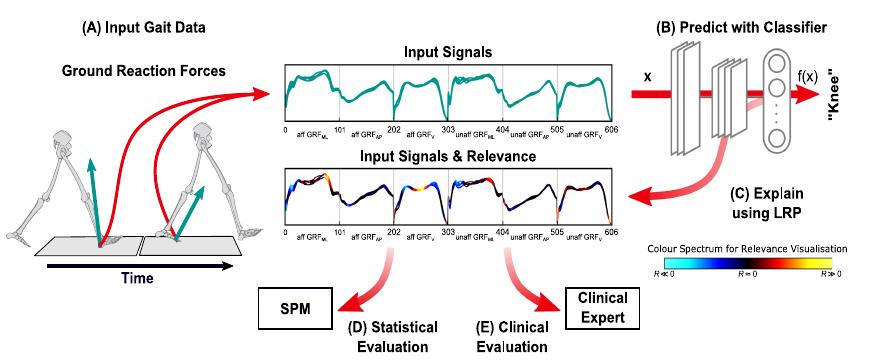
\includegraphics[width=0.8\textwidth]{Images/Slijep2023_1.jpg}
\end{figure}

%%%%%%%%%%%%%%%%%%%%%%%%%%%%%%%%%%%%%%%%%%%%%%%%%%%%%%%%%%%%%%%%%

\section{Explainable gait recognition with prototyping encoder-decoder}

\subsection{Detalles del Artículo}
\begin{itemize}
    \item \textbf{Título:} Explainable gait recognition with prototyping encoder-decoder
    \item \textbf{Autores:} Jucheol Moon, Yong-Min Shin, Jin-Duk Park, Nelson Hebert Minaya, Won-Yong Shin, Sang-Il Choi
    \item \textbf{Revista:} PLOS ONE
    \item \textbf{Nivel:} Multidisciplinaria, Cuartil Q1, índice de impacto 3.752 (2022-2023).
    \item \textbf{Fecha de publicación:} marzo de 2022.
\end{itemize}

\subsection{Problema Principal}
El artículo aborda el reconocimiento de marcha en un entorno de \textit{open set}, un desafío donde se busca identificar a individuos conocidos y rechazar a desconocidos. Este enfoque es útil en aplicaciones biométricas y médicas. Además, el trabajo resuelve problemas de sensibilidad a hiperparámetros y falta de interpretabilidad de modelos tradicionales mediante una arquitectura innovadora y herramientas de inteligencia artificial explicable (XAI).

\subsection{Creación de Datos para el Modelo}
Los datos se recolectan usando plantillas de calzado equipadas con sensores (presión, aceleración y rotación). Cada muestra es segmentada en pasos unitarios representativos, con suavizado Gaussiano aplicado para eliminar errores.

\subsection{Cálculo de Prototipos}
Los prototipos para cada sujeto se calculan promediando los vectores embebidos correspondientes a los pasos unitarios en cada modalidad (presión, aceleración y rotación). La fórmula general es:
\[
c_m^a = \frac{1}{q} \sum_{i=1}^q s_i^m
\]
donde \(c_m^a\) es el prototipo de la modalidad \(m\) para el sujeto \(a\), y \(q\) es el número total de pasos.

\subsection{Arquitectura del Modelo y Flujo de Datos}
El sistema propuesto es un prototipo de red \textit{encoder-decoder} con las siguientes características:
\begin{itemize}
    \item \textbf{Encoder:} Transforma los pasos unitarios en vectores embebidos de 128 dimensiones, empleando tres sub-\textit{encoders} con capas convolucionales 1D.
    \item \textbf{Decoder:} Reconstruye los datos originales desde los vectores embebidos. En este modelo, el decoder intenta aproximar el prototipo promedio de las muestras de un sujeto (en cada modalidad: presión, aceleración o rotación) desde el vector embebido generado por el encoder.
    \item \textbf{Funciones de pérdida:}
    \begin{itemize}
        \item \textbf{Pérdida de triplete:} Aumenta la separación entre clases distintas y reduce la dispersión dentro de una misma clase. Su expresión es:
        \[
        L_{\text{triplet}} = \|\mathbf{v}_{i,a} - \mathbf{v}_{j,a}\|^2_2 - \|\mathbf{v}_{i,a} - \mathbf{v}_{k,b}\|^2_2 + \alpha
        \]
        donde:
        \begin{itemize}
            \item \(\mathbf{v}_{i,a}\) y \(\mathbf{v}_{j,a}\): vectores embebidos de pasos unitarios del mismo sujeto \(a\),
            \item \(\mathbf{v}_{k,b}\): vector embebido de un paso unitario de un sujeto distinto \(b\),
            \item \(\alpha\): margen que define la separación mínima deseada.
        \end{itemize}
        \item \textbf{Pérdida de prototipo:} Reduce la distancia entre los datos originales y sus prototipos promedio. Su expresión es:
        \[
        L_{\text{proto}} = \frac{1}{|M|} \sum_{m \in M} \|g(f(s^m_{i,a})) - c^m_a\|^2_2
        \]
        donde:
        \begin{itemize}
            \item \(g(f(s^m_{i,a}))\): reconstrucción del prototipo por el \textit{decoder},
            \item \(c^m_a\): prototipo promedio de la modalidad \(m\) para el sujeto \(a\),
            \item \(M\): conjunto de modalidades (presión, aceleración, rotación).
        \end{itemize}
    \end{itemize}
\end{itemize}

\subsection{Interpretabilidad del Modelo (XAI)}

El modelo utiliza herramientas de XAI para producir explicaciones visuales y cuantitativas:

\begin{itemize}
    \item \textbf{Mapas de atribución (heatmaps):}
    \begin{itemize}
        \item Representan la relevancia de cada característica de entrada (presión, aceleración, rotación) en el tiempo.
        \item Se visualizan como mapas de calor donde:
        \begin{itemize}
            \item El eje horizontal representa las características.
            \item El eje vertical representa el tiempo.
            \item Los colores más intensos indican mayor relevancia.
        \end{itemize}
    \end{itemize}
    \item \textbf{Pruebas de degradación del desempeño:}
    \begin{itemize}
        \item Ocultan áreas identificadas como relevantes por los mapas de atribución.
        \item Evalúan cómo disminuye el desempeño del modelo (medido por precisión, TPR y TNR) al eliminar esas áreas.
    \end{itemize}
\end{itemize}

\textbf{Métodos empleados:}
\begin{itemize}
    \item \textbf{Análisis de Sensibilidad (SA):} Mide cómo pequeños cambios en el input afectan la salida.
    \item \textbf{Propagación de Relevancia por Capas (LRP):} Redistribuye la relevancia de la salida hacia las entradas para identificar características críticas.
\end{itemize}

\textbf{Tipo de explicaciones:}
\begin{itemize}
    \item \textbf{Gráficas:} Mapas de calor y degradación del desempeño.
    \item \textbf{Cuantitativas:} Valores numéricos que indican sensibilidad y relevancia.
\end{itemize}

\subsection{Uso Práctico del Modelo}
El flujo operativo para reconocimiento incluye:
\begin{enumerate}
    \item \textbf{Codificación:} Un paso unitario es mapeado al espacio latente mediante el \textit{encoder}.
    \item \textbf{Comparación:} El vector embebido es comparado con prototipos conocidos usando una máquina de soporte vectorial (\textit{OSVM}).
    \item \textbf{Decisión:} Si el vector cae dentro del límite de decisión, se clasifica como una clase conocida; de lo contrario, se rechaza.
\end{enumerate}


\subsection{Resultados y Evaluación}
\begin{itemize}
    \item \textbf{Desempeño:} El sistema logra métricas de precisión (\textit{ACC}), tasa de verdaderos positivos (\textit{TPR}) y tasa de verdaderos negativos (\textit{TNR}) superiores al 90\%.
    \item \textbf{Robustez:} La combinación de pérdidas reduce la dependencia del modelo a los hiperparámetros.
    \item \textbf{Explicabilidad:} Los mapas de atribución revelan qué partes de los datos (como fases de contacto con el suelo) son más relevantes para la clasificación.
\end{itemize}

\begin{figure}[H] 
    \centering
    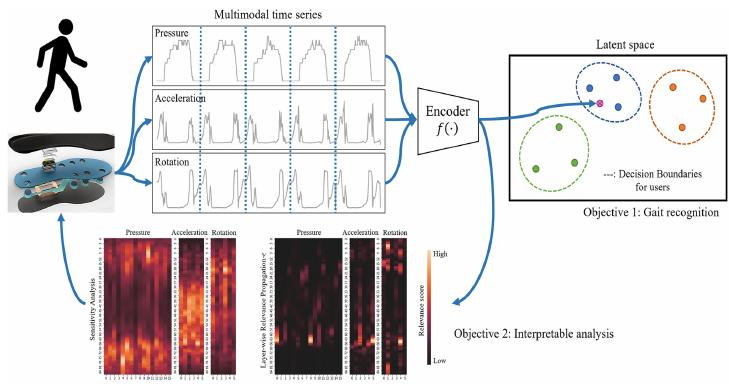
\includegraphics[width=0.5\textwidth]{Images/Moon2022_1.jpg}
    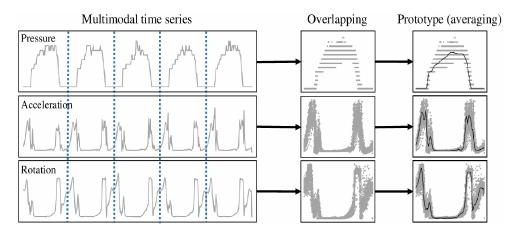
\includegraphics[width=0.4\textwidth]{Images/Moon2022_2.jpg}
    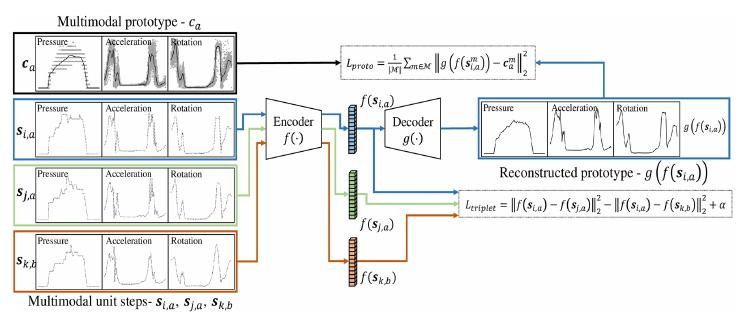
\includegraphics[width=0.4\textwidth]{Images/Moon2022_3.jpg}
    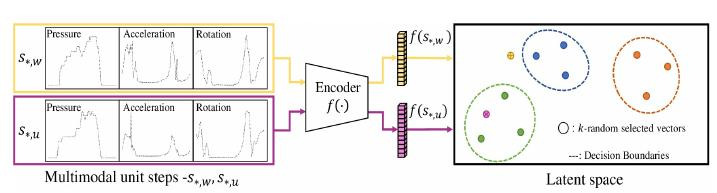
\includegraphics[width=0.5\textwidth]{Images/Moon2022_4.jpg}
    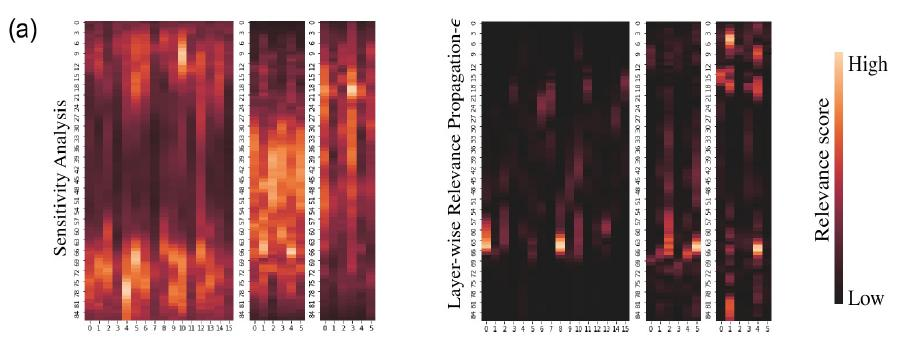
\includegraphics[width=0.4\textwidth]{Images/Moon2022_5.jpg}
    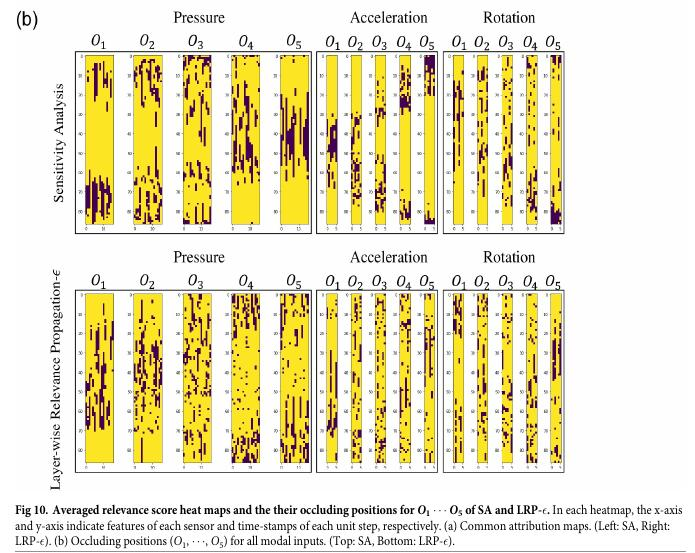
\includegraphics[width=0.4\textwidth]{Images/Moon2022_6.jpg}
\end{figure}

%%%%%%%%%%%%%%%%%%%%%%%%%%%%%%%%%%%%%%%%%%%%%%%%%%%%%%%%%%%%%%%%%%%%%%%%%%%%%%%%%%%%%%%

\section{XAI and Wearable Sensor-Based Gait Analysis to Identify Patients with Osteopenia and Sarcopenia in Daily Life}

\subsection{Detalles del Artículo}
\begin{itemize}
    \item \textbf{Título:} XAI and Wearable Sensor-Based Gait Analysis to Identify Patients with Osteopenia and Sarcopenia in Daily Life
    \item \textbf{Autores:} Jeong-Kyun Kim, Myung-Nam Bae, Kangbok Lee, Jae-Chul Kim, Sang Gi Hong
    \item \textbf{Revista:} Biosensors
    \item \textbf{Nivel:} Revista revisada por pares, cuartil Q2 en bioingeniería y tecnologías de sensores.
    \item \textbf{Fecha de publicación:} marzo de 2022.
\end{itemize}

\subsection{Problema Principal}
El artículo busca identificar pacientes con osteopenia y sarcopenia utilizando análisis de marcha basado en sensores inerciales. Este enfoque permite evaluar el riesgo de estas condiciones en la vida diaria sin necesidad de equipamiento médico especializado. Además, el estudio utiliza inteligencia artificial explicable (XAI) para analizar la relevancia de los parámetros de marcha en las decisiones del modelo.

\subsection{Arquitectura del Modelo}
Se emplearon múltiples modelos de aprendizaje automático y aprendizaje profundo:
\begin{itemize}
    \item \textbf{Modelos ML:}
    \begin{itemize}
        \item Random Forest (RF)
        \item Extreme Gradient Boosting (XGBoost)
        \item Máquina de Soporte Vectorial (SVM)
    \end{itemize}
    \item \textbf{Modelos DL:}
    \begin{itemize}
        \item Convolutional Neural Network (CNN)
        \item Bi-Directional Long Short-Term Memory (BiLSTM)
        \item ResNet50 con transferencia de aprendizaje
    \end{itemize}
    \item \textbf{Explicabilidad:} Uso de SHAP, Grad-CAM y Relevance-CAM para interpretar la contribución de los parámetros al modelo.
\end{itemize}

\subsection{Creación y Preprocesamiento de Datos}
\begin{itemize}
    \item \textbf{Participantes:} 42 mujeres mayores de 65 años:
    \begin{itemize}
        \item 21 pacientes con osteopenia y 21 sin osteopenia.
        \item 10 pacientes con sarcopenia y 10 sin sarcopenia.
    \end{itemize}
    \item \textbf{Datos:} Señales inerciales recolectadas mediante plantillas con sensores IMU.
    \item \textbf{Parámetros:}
    \begin{itemize}
        \item 24 parámetros espacio-temporales (e.g., fase de soporte, fase de balanceo, cadencia).
        \item 100 parámetros estadísticos descriptivos (e.g., promedio, desviación estándar, curtosis).
    \end{itemize}
\end{itemize}

\subsection{Resultados y Métricas}
\begin{itemize}
    \item \textbf{Osteopenia:}
    \begin{itemize}
        \item \textbf{XGBoost:} Precisión de 88.69\% con los 4 parámetros más relevantes.
        \item \textbf{ResNet (transfer learning):} Precisión de 78.6\%, F1-score de 78.7\%.
    \end{itemize}
    \item \textbf{Sarcopenia:}
    \begin{itemize}
        \item \textbf{RF:} Precisión de 93.75\% con los 18 parámetros más relevantes.
        \item \textbf{ResNet (transfer learning):} Precisión de 70\%, F1-score de 60.6\%.
    \end{itemize}
\end{itemize}

\subsection{Conclusiones Clave}
\begin{itemize}
    \item Los modelos ML superaron a los modelos DL en la clasificación de osteopenia y sarcopenia.
    \item Los parámetros estadísticos descriptivos fueron más informativos que los parámetros espacio-temporales.
    \item XAI proporcionó explicaciones detalladas de cómo los parámetros contribuyen al diagnóstico, mejorando la confiabilidad del modelo.
\end{itemize}

\begin{figure}[H] 
    \centering
    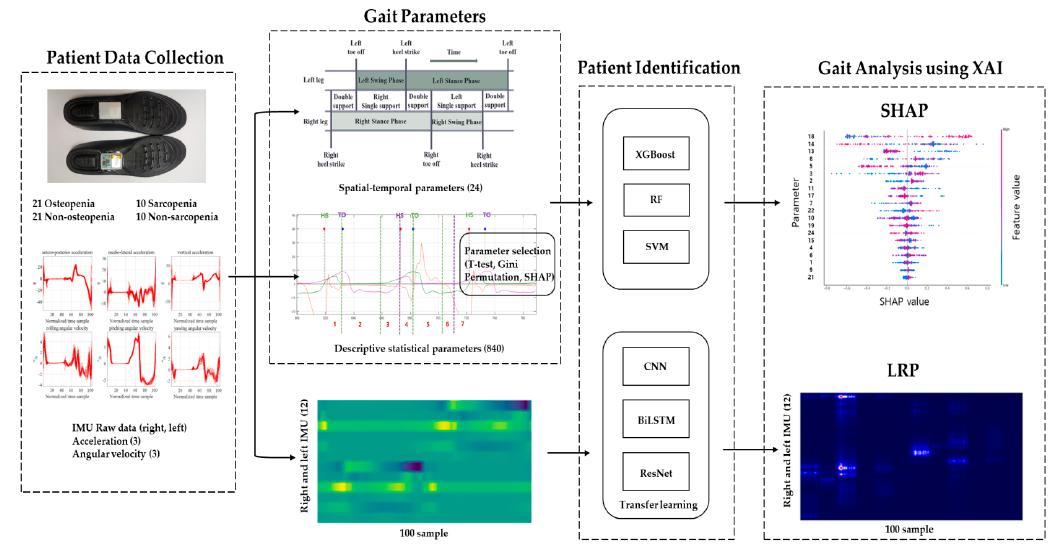
\includegraphics[width=0.8\textwidth]{Images/Kim2022.jpg}
\end{figure}

%%%%%%%%%%%%%%%%%%%%%%%%%%%%%%%%%%%%%%%%%%%%%%%%%%%%%%%%%%%%%%%%%%%%%%%%%%%%%

\section{Leveraging Explainable Machine Learning to Identify Gait Biomechanical Parameters Associated with ACL Injury}

\subsection{Detalles del Artículo}
\begin{itemize}
    \item \textbf{Título:} Leveraging Explainable Machine Learning to Identify Gait Biomechanical Parameters Associated with Anterior Cruciate Ligament Injury
    \item \textbf{Autores:} Christos Kokkotis, Serafeim Moustakidis, Themistoklis Tsatalas, et al.
    \item \textbf{Revista:} Scientific Reports
    \item \textbf{Nivel:} Publicación revisada por pares, cuartil Q1 en multidisciplinario.
    \item \textbf{Fecha de publicación:} abril de 2022.
\end{itemize}

\subsection{Problema Principal}
El artículo aborda la identificación de parámetros biomecánicos relevantes para diagnosticar lesiones del ligamento cruzado anterior (ACL) y evaluar la efectividad de la reconstrucción (ACLR). Se utiliza aprendizaje automático explicable (XAI) para superar la opacidad de los modelos tradicionales y vincular parámetros biomecánicos a resultados clínicos.

\subsection{Arquitectura del Modelo}
Se diseñó un pipeline de aprendizaje automático con los siguientes componentes:
\begin{itemize}
    \item \textbf{Selección de características:} ReliefF para reducir la dimensionalidad del espacio de características.
    \item \textbf{Modelos ML evaluados:}
    \begin{itemize}
        \item \textbf{SVM:} Mejor desempeño con \textbf{Accuracy} de 94.95\%.
        \item \textbf{Red Neuronal (NN):} Segundo mejor desempeño con \textbf{Accuracy} de 92.89\%.
        \item Otros modelos evaluados: XGBoost, Random Forest, Decision Trees, Logistic Regression, Naive Bayes, KNN.
    \end{itemize}
    \item \textbf{Explicabilidad:} SHAP para analizar el impacto de cada característica en la salida del modelo.
\end{itemize}

\subsection{Creación y Preprocesamiento de Datos}
\begin{itemize}
    \item \textbf{Participantes:} 151 sujetos divididos en tres grupos:
    \begin{itemize}
        \item CON: Controles sanos.
        \item ACLD: Pacientes con ACL lesionado.
        \item ACLR: Pacientes después de reconstrucción de ACL.
    \end{itemize}
    \item \textbf{Datos recolectados:} Fuerzas de reacción al suelo (GRF), cinemática y cinética del plano sagital.
    \item \textbf{Normalización:} Escalado a [0,1] y uso de técnicas de filtrado de datos.
\end{itemize}

\subsection{Resultados y Métricas}
\begin{itemize}
    \item \textbf{Clasificación Multiclase (CON, ACLD, ACLR):}
    \begin{itemize}
        \item SVM: Mejor desempeño global con \textbf{Accuracy} de 94.95\%, Precision de hasta 96.72\% y Recall de hasta 97.62\%.
        \item NN: Accuracy de 92.89\%.
    \end{itemize}
    \item \textbf{Principales parámetros identificados (SHAP):} K2, H4, A3, GRF4, GRF7, K1, A4.
    \item \textbf{Estadística:} Diferencias significativas en parámetros como K2, H4 y GRF4, confirmadas mediante ANOVA.
\end{itemize}

\subsection{Conclusiones Clave}
\begin{itemize}
    \item Los modelos XAI permiten identificar parámetros biomecánicos que los análisis estadísticos tradicionales podrían ignorar.
    \item Parámetros como el ángulo mínimo de flexión de rodilla (K2) y el momento máximo de flexión de cadera (H4) están vinculados a resultados clínicos.
    \item Se destaca la necesidad de herramientas más robustas para interpretar interacciones complejas entre parámetros.
\end{itemize}

%%%%%%%%%%%%%%%%%%%%%%%%%%%%%%%%%%%%%%%%%%%%%

\section{Trustworthy Visual Analytics in Clinical Gait Analysis}

\subsection{Detalles del Artículo}
\begin{itemize}
    \item \textbf{Título:} Trustworthy Visual Analytics in Clinical Gait Analysis: A Case Study for Patients with Cerebral Palsy
    \item \textbf{Autores:} Alexander Rind, Djordje Slijepčević, Matthias Zeppelzauer, Fabian Unglaube, Andreas Kranzl, Brian Horsak
    \item \textbf{Revista:} IEEE Workshop on Trust and Expertise in Visual Analytics (TREX)
    \item \textbf{Nivel:} Publicación revisada por pares en un taller de la IEEE.
    \item \textbf{Fecha de publicación:} 19 de diciembre de 2022.
\end{itemize}

\subsection{Problema Principal}
El análisis clínico de la marcha en pacientes con parálisis cerebral (PC) produce grandes cantidades de datos complejos. Los modelos de aprendizaje automático han demostrado ser útiles para clasificar patrones de marcha, pero su naturaleza de caja negra genera desconfianza entre los clínicos. El artículo propone una solución de analítica visual enriquecida con explicabilidad (gaitXplorer) para aumentar la transparencia y confianza en los modelos.

\subsection{Arquitectura del Modelo}
\begin{itemize}
    \item \textbf{Datos:} 
    \begin{itemize}
        \item Datos tridimensionales de análisis de marcha de 257 niños (355 extremidades afectadas) con PC.
        \item Variables como ángulos articulares, momentos articulares y fuerzas de reacción del suelo (GRF).
    \end{itemize}
    \item \textbf{Modelo:} 
    \begin{itemize}
        \item Red Neuronal Convolucional (CNN) de una dimensión.
        \item Estructura: 4 capas convolucionales seguidas de capas totalmente conectadas y una capa \textit{softmax} con cuatro clases de salida (true equinus, jump gait, apparent equinus y crouch gait).
        \item Función de activación: SELU, con regularización por \textit{alpha dropout}.
    \end{itemize}
    \item \textbf{Explicabilidad:} 
    \begin{itemize}
        \item Algoritmo Grad-CAM adaptado para datos unidimensionales.
        \item Identifica regiones relevantes de las series temporales que contribuyen a las predicciones.
    \end{itemize}
\end{itemize}

\subsection{Interfaz Visual Interactiva}
\begin{itemize}
    \item Interfaz basada en web que permite:
    \begin{itemize}
        \item Visualizar las series temporales de un paciente y su relevancia en las predicciones.
        \item Comparar datos de un paciente con grupos promedio.
        \item Modificar clasificaciones automáticas.
    \end{itemize}
    \item Los datos se presentan en gráficos de líneas organizados por variables biomecánicas y partes del cuerpo.
    \item Tres modos de visualización:
    \begin{itemize}
        \item Modo estándar: Muestra datos promedio.
        \item Modo de explicabilidad: Resalta regiones relevantes usando Grad-CAM.
        \item Modo de comparación grupal: Compara al paciente con promedios de grupos clasificados.
    \end{itemize}
\end{itemize}

\subsection{Evaluación de las Explicaciones}
\begin{itemize}
    \item Se realizó un estudio de caso con dos expertos clínicos que evaluaron ocho pacientes.
    \item Feedback:
    \begin{itemize}
        \item Se confiaron en explicaciones para cuatro extremidades, mientras que otras fueron consideradas sospechosas por falta de relevancia en áreas esperadas.
        \item Ejemplo: Para true equinus, los expertos esperaban alta relevancia en el ángulo sagital del tobillo, pero el modelo destacó el ángulo sagital de la rodilla.
    \end{itemize}
    \item Las explicaciones fueron calificadas como esenciales para ganar confianza en las clasificaciones automáticas.
\end{itemize}

\subsection{Conclusiones Clave}
\begin{itemize}
    \item La integración de Grad-CAM y visualizaciones interactivas mejora la transparencia de los modelos de aprendizaje automático.
    \item Se identificaron discrepancias entre las expectativas clínicas y las explicaciones generadas, subrayando la necesidad de mejorar los algoritmos explicables.
    \item El enfoque propuesto tiene potencial para generalizarse a otros contextos clínicos y sistemas de análisis visual.
\end{itemize}

\begin{figure}[H] 
    \centering
    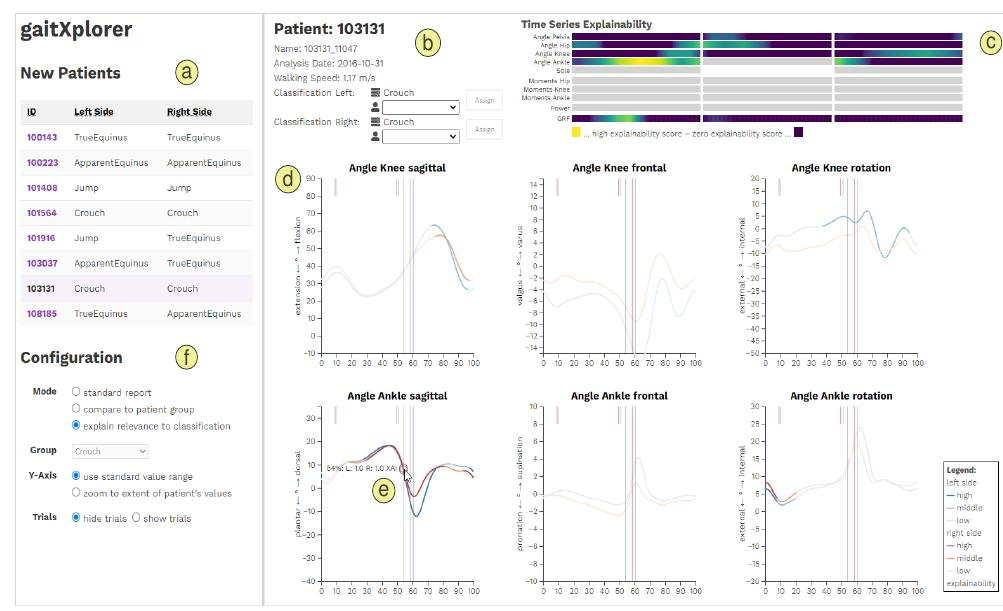
\includegraphics[width=0.8\textwidth]{Images/Rind2022.jpg}
\end{figure}



%%%%%%%%%%%%%%%%%%%%%%%%%%%%%%%%%%%%%%%%%%%%%

\section{Explainable Machine Learning in Human Gait Analysis: A Study on Children With Cerebral Palsy}

\subsection{Detalles del Artículo}
\begin{itemize}
    \item \textbf{Título:} Explainable Machine Learning in Human Gait Analysis: A Study on Children With Cerebral Palsy
    \item \textbf{Autores:} Djordje Slijepcevic, Matthias Zeppelzauer, Fabian Unglaube, Andreas Kranzl, Christian Breiteneder, Brian Horsak
    \item \textbf{Revista:} IEEE Access
    \item \textbf{Nivel:} Revista revisada por pares, cuartil Q1 en ingeniería y ciencias de la computación.
    \item \textbf{Fecha de publicación:} junio de 2023.
\end{itemize}

\subsection{Problema Principal}
El estudio aborda la clasificación de patrones de marcha asociados con la parálisis cerebral (CP) mediante datos de análisis de marcha 3D clínicos (3DGA). Además, utiliza métodos de explicabilidad (XAI) para evaluar la relevancia clínica de las características aprendidas por los modelos, enfrentando los desafíos de opacidad y aceptación clínica de los modelos de aprendizaje automático.

\subsection{Arquitectura del Modelo}
Se evaluaron cuatro tipos de modelos:
\begin{itemize}
    \item \textbf{Modelos de aprendizaje profundo:}
    \begin{itemize}
        \item Redes Neuronales Convolucionales (CNNs)
        \item Redes Neuronales Auto-normalizantes (SNNs)
    \end{itemize}
    \item \textbf{Modelos tradicionales:}
    \begin{itemize}
        \item Random Forest (RF)
        \item Decision Trees (DT)
    \end{itemize}
\end{itemize}

\subsection{Datos y Preprocesamiento}
\begin{itemize}
    \item \textbf{Conjunto de datos:} 302 pacientes (375 extremidades afectadas) categorizados en cuatro patrones de marcha (true equinus, crouch gait, jump gait, apparent equinus).
    \item \textbf{Captura de datos:} Señales cinemáticas y de fuerzas de reacción al suelo (GRF), normalizadas a un ciclo de marcha completo.
    \item \textbf{Configuraciones de entrada:}
    \begin{itemize}
        \item Todas las señales de 3DGA.
        \item Solo señales cinemáticas.
        \item Ángulos sagitales de rodilla y tobillo.
        \item Solo señales de GRF.
    \end{itemize}
\end{itemize}

\subsection{Métodos XAI y Aplicaciones Prácticas}
\begin{itemize}
    \item \textbf{Métodos utilizados:}
    \begin{itemize}
        \item \textbf{Grad-CAM:}
        \begin{itemize}
            \item Utilizado con CNNs para generar mapas de saliencia que destacan las regiones de las señales más relevantes para la clasificación.
            \item Los mapas ayudan a identificar cuáles partes del ciclo de marcha (e.g., fase de soporte, oscilación) son clave para las predicciones del modelo.
        \end{itemize}
        \item \textbf{Importancia de características (Gini Impurity):}
        \begin{itemize}
            \item Aplicado en modelos RF y DT para medir la relevancia de cada característica (e.g., ángulos sagitales, GRF).
            \item Los valores más altos indican las características más críticas para el modelo.
        \end{itemize}
    \end{itemize}
    \item \textbf{Uso práctico:}
    \begin{itemize}
        \item Grad-CAM permitió a los clínicos visualizar directamente qué fases y señales específicas de la marcha influyeron en las predicciones del modelo.
        \item La importancia de características permitió identificar parámetros biomecánicos clave como los ángulos sagitales de tobillo y rodilla, orientando la evaluación clínica hacia esas señales.
        \item Estas explicaciones respaldan decisiones clínicas, facilitando la comprensión del diagnóstico y la planificación del tratamiento.
    \end{itemize}
\end{itemize}

\subsection{Resultados y Métricas}
\begin{itemize}
    \item \textbf{Mejor desempeño:} Random Forest con precisión de \textbf{93.4\%} utilizando ángulos sagitales de rodilla y tobillo.
    \item \textbf{Comparación de modelos:} 
    \begin{itemize}
        \item CNNs y SNNs muestran menor precisión y mayor sensibilidad a configuraciones de entrada.
        \item Los modelos tradicionales (RF y DT) se enfocan en características clínicamente relevantes con explicaciones más concisas.
    \end{itemize}
    \item \textbf{Explicabilidad:} Grad-CAM destaca regiones temporales en las señales, mientras que los modelos basados en árboles muestran la jerarquía de importancia de características.
\end{itemize}

\subsection{Conclusiones Clave}
\begin{itemize}
    \item Los modelos tradicionales superan a las redes neuronales en precisión y robustez.
    \item Los métodos XAI destacan la relevancia de las señales sagitales (rodilla y tobillo) como características clave para la clasificación.
    \item La integración de explicabilidad promueve la confianza en los modelos y su potencial uso en la práctica clínica.
\end{itemize}

%%%%%%%%%%%%%%%%%%%%%%%%%%%%%%%%%%%%%%%%%%%%%%%%%%%%%%%%%%%%%%%%%%%%%%%%%%%%%%%%%%%%%%%%%%%

\section{A New Method Applied for Explaining the Landing Patterns}

\subsection{Detalles del Artículo}
\begin{itemize}
    \item \textbf{Título:} A New Method Applied for Explaining the Landing Patterns: Interpretability Analysis of Machine Learning
    \item \textbf{Autores:} Datao Xu, Huiyu Zhou, Wenjing Quan, Ukadike Chris Ugbolue, Fekete Gusztav, Yaodong Gu
    \item \textbf{Revista:} Heliyon
    \item \textbf{Nivel:} Revista de acceso abierto revisada por pares, cuartil Q1 en ciencias multidisciplinarias.
    \item \textbf{Fecha de publicación:} 9 de febrero de 2024.
\end{itemize}

\subsection{Problema Principal}
El artículo aborda la falta de interpretabilidad en los modelos de aprendizaje automático utilizados para reconocer patrones de aterrizaje en biomecánica clínica. Proponen un modelo basado en \textit{Layer-wise Relevance Propagation} (LRP) que no solo mejora la transparencia, sino que también identifica las características más relevantes de las señales biomecánicas.

\subsection{Arquitectura del Modelo}
\begin{itemize}
    \item \textbf{Modelos evaluados:} SVM, ANN, CNN y ZeroR.
    \item \textbf{Modelo final:} Red Neuronal Artificial (ANN) con el mejor rendimiento.
    \item \textbf{Datos de entrada:}
    \begin{itemize}
        \item Señales cinemáticas y cinéticas tridimensionales de las extremidades inferiores durante la fase de aterrizaje.
        \item Datos segmentados por articulación (tobillo, rodilla, cadera) y por plano (sagital, frontal, transversal).
    \end{itemize}
\end{itemize}

\subsection{Evaluación de las Explicaciones}
\begin{itemize}
    \item \textbf{Método de explicabilidad:} 
    \begin{itemize}
        \item LRP: Calcula puntajes de relevancia (\textit{Relevance Scores}, RS) para identificar la contribución de cada característica de entrada.
    \end{itemize}
    \item \textbf{Evaluación estadística:}
    \begin{itemize}
        \item \textit{Statistical Parametric Mapping (SPM):} Verifica diferencias significativas entre patrones utilizando pruebas t pareadas.
        \item Tamaño del efecto (\textit{Effect Size}): Mide la magnitud de las diferencias en las señales relevantes.
    \end{itemize}
    \item \textbf{Resultados clave:}
    \begin{itemize}
        \item Consistencia entre los RS derivados del LRP y los resultados estadísticos en las articulaciones del tobillo y la rodilla.
        \item Mayor relevancia en las señales del plano sagital y durante las primeras fases del aterrizaje.
    \end{itemize}
\end{itemize}

\subsection{Resultados de Clasificación}
\begin{itemize}
    \item \textbf{Desempeño de modelos:}
    \begin{itemize}
        \item ANN obtuvo una precisión promedio de 99.46\% con señales combinadas (cinemática y cinética).
        \item Mejor clasificación observada para datos de la rodilla y el plano sagital.
    \end{itemize}
\end{itemize}

\subsection{Conclusiones Clave}
\begin{itemize}
    \item El modelo basado en LRP permite una comprensión más profunda de las contribuciones específicas de cada señal al reconocimiento de patrones de aterrizaje.
    \item El enfoque propuesto puede mejorar significativamente la confianza y transparencia en aplicaciones clínicas.
\end{itemize}

\begin{figure}[H] 
    \centering
    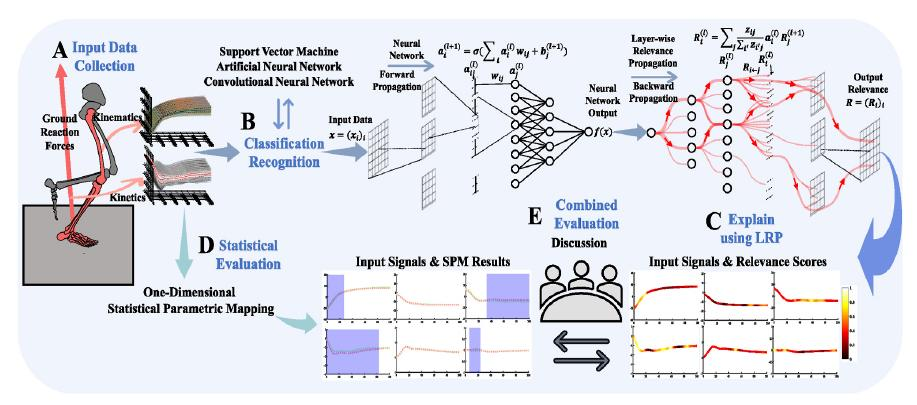
\includegraphics[width=0.9\textwidth]{Images/Xu.jpg}
\end{figure}


%%%%%%%%%%%%%%%%%%%%%%%%%%%%%%%%%%%%%%%%%%%%%%%%%%%%%%%%%%%%%%%%%%%%%%%%%%%%%%%%%%%%%%%%%
\section{Identification and Interpretation of Gait Analysis Features and Foot Conditions by Explainable AI}

\subsection{Detalles del Artículo}
\begin{itemize} 
    \item \textbf{Título:} Identification and Interpretation of Gait Analysis Features and Foot Conditions by Explainable AI
    \item \textbf{Autores:} Mustafa Erkam Özateş, Alper Yaman, Firooz Salami, Sarah Campos, Sebastian I. Wolf, Urs Schneider
    \item \textbf{Revista:} Scientific Reports
    \item \textbf{Nivel:} Revista revisada por pares, cuartil Q1, índice de impacto 4.996 (2023).
    \item \textbf{Fecha de publicación:} marzo de 2024.
\end{itemize}

\subsection{Problema Principal}
El artículo aborda la complejidad del análisis clínico de la marcha, un proceso crítico para diagnosticar condiciones del pie y planificar cirugías. Propone un pipeline de aprendizaje automático (ML) e inteligencia artificial explicable (XAI) para la selección de características y la identificación automática de condiciones específicas del pie.


\begin{figure}[H] 
    \centering
    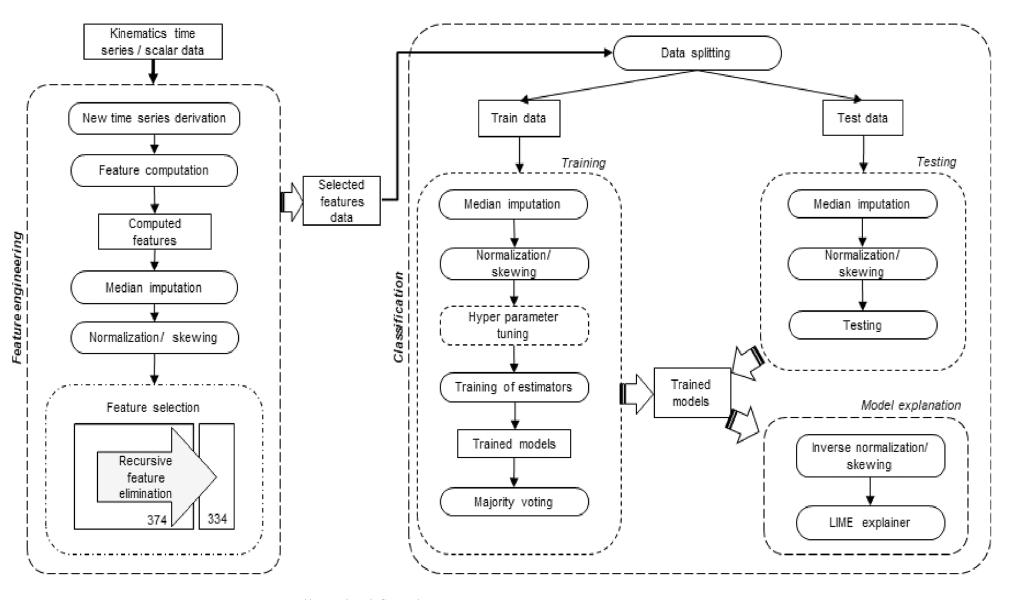
\includegraphics[width=0.8\textwidth]{Images/Erkam2024_1.jpg}
\end{figure}

\subsection{Arquitectura del Modelo}
Se evaluaron cinco modelos de ML:
\begin{itemize}
    \item \textbf{Support Vector Machines (SVM):} Modelo base para selección de características.
    \item \textbf{Random Forest (RF):} Modelo robusto contra desequilibrio de clases.
    \item \textbf{Logistic Regression (LREG):} Modelo lineal supervisado.
    \item \textbf{K-nearest Neighbors (KNN):} Clasificador basado en distancias.
    \item \textbf{Majority Voting (MV):} Combina los modelos anteriores con votación ponderada.
\end{itemize}

\subsection{Creación y Preprocesamiento de Datos}
\begin{itemize}
    \item \textbf{Dataset:} 348 sujetos (248 pacientes con 6 condiciones específicas del pie y 100 sujetos control).
    \item \textbf{Ángulos funcionales analizados:} 12 ángulos derivados de un ciclo de marcha (ej. flexión tibiotalar, ángulo del arco medial).
    \item \textbf{Normalización:} Los datos se normalizaron entre 0 y 1, y se imputaron valores faltantes con la mediana.
    \item \textbf{Extracción de características:} Se generaron 374 características, incluyendo derivadas temporales y desviaciones respecto a patrones normales.
    \item \textbf{Selección de características:} Eliminación recursiva de características basada en SVM y RF, reduciendo el conjunto a 334 características.
\end{itemize}

\subsection{Resultados}
\begin{itemize}
    \item \textbf{Mejores desempeños:}
    \begin{itemize}
        \item \textbf{KNN y MV:} Precisión balanceada (\textbf{Balanced Accuracy}), \textbf{Recall}, \textbf{Precision} y \textbf{F1 Score} promedio de 0.87.
        \item Otros modelos alcanzaron métricas superiores a 0.82 en promedio.
    \end{itemize}
    \item \textbf{Interpretación con LIME:}
    \begin{itemize}
        \item Identificación de las cinco características más relevantes por condición del pie.
        \item Ejemplo: En \textit{tibiotalar osteoarthritis}, el ángulo mínimo del arco medial fue crítico en las fases de soporte y oscilación.
    \end{itemize}
\end{itemize}

\subsection{Conclusiones}
El pipeline propuesto demuestra que la combinación de ML y XAI puede automatizar y mejorar la interpretación del análisis de marcha, ofreciendo una herramienta útil para médicos al identificar características relevantes y condiciones específicas del pie.
%%%%%%%%%%%%%%%%%%%%%%%%%%%%%%%%%%%%%%%%%%%%%%%%%%%%%%%%



%%%%%%%%%%%%%%%%%%%%%%%%%%%%%%%%%%%%%%%%%%%%%%%%%%%%%%
%%%%%%%%%%%%%%%%%%%%%%%%%%%%%%%%%%%%%%%%%%%%%%%%%%%%%%%
\chapter{Otros}

\section{Assessing Fidelity in XAI Post-hoc Techniques: A Comparative Study with Ground Truth Explanations Datasets}

\subsection{Detalles del Artículo}
\begin{itemize}
    \item \textbf{Título:} Assessing Fidelity in XAI Post-hoc Techniques: A Comparative Study with Ground Truth Explanations Datasets
    \item \textbf{Autores:} Miquel Miró-Nicolau, Antoni Jaume-i-Capó, Gabriel Moyà-Alcover
    \item \textbf{Revista:} Preprint, arXiv
    \item \textbf{Nivel:} Investigación preliminar sin revisión por pares.
    \item \textbf{Fecha de publicación:} Noviembre de 2023.
\end{itemize}

\subsection{Problema Principal}
El artículo aborda la necesidad de evaluar la fidelidad de los métodos de explicabilidad de IA (XAI) post-hoc en comparación con los modelos originales. Dado que no existe una ground truth en explicaciones generadas, se diseñan datasets sintéticos con explicaciones controladas para validar la precisión y consistencia de los métodos XAI.

\subsection{Definición de Fidelidad}
En este artículo, la fidelidad se define como la capacidad de un método XAI para representar de manera precisa las características relevantes que el modelo utiliza para tomar decisiones. En otras palabras, un método es fiel si las explicaciones generadas reflejan de manera confiable los patrones o regiones importantes identificadas por el modelo original durante su proceso de inferencia.

\subsection{Metodología}
\begin{itemize}
    \item \textbf{Conjuntos de datos:} 
    \begin{itemize}
        \item Creación de los datasets TXUXIv1, TXUXIv2, y TXUXIv3 con diferentes niveles de complejidad visual.
        \item Las imágenes incluyen ground truth generadas a partir de máscaras controladas, diseñadas para evaluar la correspondencia entre explicaciones y patrones reales.
    \end{itemize}
    \item \textbf{Modelos:} Red Neuronal Convolucional (CNN) preentrenada para tareas de clasificación y regresión.
    \item \textbf{Métricas de evaluación:}
    \begin{itemize}
        \item \textbf{Earth Mover’s Distance (EMD):} Mide qué tan diferentes son las distribuciones de saliencia generadas por el método XAI y las "verdades terreno".
        \item \textbf{Minimum Intersection over Union (MIN):} Evalúa la superposición entre los mapas de saliencia generados y las regiones reales relevantes.
    \end{itemize}
\end{itemize}

\subsection{Comparación de Métodos XAI}
Se evaluaron 13 métodos de explicabilidad post-hoc, divididos en tres categorías:
\begin{itemize}
    \item \textbf{Métodos de sensibilidad:} LIME, SHAP, RISE.
    \item \textbf{Métodos basados en Class Activation Maps (CAM):} Grad-CAM, Grad-CAM++, Score-CAM, SIDU.
    \item \textbf{Métodos de retropropagación:} Gradient, Guided Backpropagation (GBP), Layer-wise Relevance Propagation (LRP), DeepLIFT, Integrated Gradients, SmoothGrad.
\end{itemize}

\subsection{Evaluación de las Explicaciones}
\begin{itemize}
    \item \textbf{Resultados en EMD:} 
    \begin{itemize}
        \item Los métodos GBP y LRP obtuvieron los valores más bajos (mejor desempeño), con \(EMD \leq 0.035\), indicando alta similitud entre las explicaciones generadas y las "verdades terreno".
        \item Métodos como LIME y SHAP presentaron mayores diferencias, lo que sugiere limitaciones en contextos con características visuales complejas.
    \end{itemize}
    \item \textbf{Resultados en MIN:}
    \begin{itemize}
        \item GBP y LRP alcanzaron los mejores valores, con \(MIN \geq 0.202\), demostrando una alta superposición con las regiones relevantes del dataset.
        \item Los métodos CAM tuvieron menores puntuaciones debido a mapas de saliencia menos precisos y difusos.
    \end{itemize}
    \item \textbf{Observaciones cualitativas:}
    \begin{itemize}
        \item Métodos basados en retropropagación generaron mapas más ruidosos pero mejor alineados con las regiones relevantes.
        \item Métodos basados en perturbación (LIME, SHAP) mostraron inconsistencias en imágenes con patrones complejos.
    \end{itemize}
\end{itemize}

\subsection{Resultados y Métricas}
\begin{itemize}
    \item Métodos basados en retropropagación (GBP, LRP) destacan por su fidelidad, especialmente en escenarios donde la complejidad de las imágenes aumenta.
    \item Métodos como SHAP y Grad-CAM se desempeñaron peor en EMD y MIN debido a la falta de consistencia en sus explicaciones.
\end{itemize}

\subsection{Conclusiones Clave}
\begin{itemize}
    \item Los métodos de retropropagación demostraron ser los más fieles, capturando con precisión las características relevantes para la toma de decisiones del modelo.
    \item Los datasets TXUXI proporcionaron una plataforma confiable para evaluar métodos XAI en escenarios controlados y realistas.
    \item Se destaca la necesidad de reducir el ruido en mapas de saliencia para mejorar la interpretabilidad y confianza de los usuarios finales.
\end{itemize}

%%%%%%%%%%%%%%%%%%%%%%%%%%%%%%%%%%%%%%%%%%%%%%%%%%%%%%%%%%%%%%%%%%%%%%%%%%%%%%%%

\section{Deep Learning for Case-Based Reasoning through Prototypes}

    \subsection{Detalles del Artículo}
    \begin{itemize}
        \item \textbf{Título:} Deep Learning for Case-Based Reasoning through Prototypes
        \item \textbf{Autores:} Oscar Li, Hao Liu, Chaofan Chen, Cynthia Rudin
        \item \textbf{Revista:} Presentado en la Trigésima Segunda Conferencia de la AAAI sobre Inteligencia Artificial (AAAI-18).
        \item \textbf{Nivel:} Investigación de alto impacto en interpretabilidad de redes neuronales.
        \item \textbf{Fecha de publicación:} 2018 (presentado como preprint en arXiv el 21 de noviembre de 2017).
    \end{itemize}

    \subsection{Problema Principal}
    El artículo aborda la falta de interpretabilidad en redes neuronales profundas, presentando una arquitectura que combina el aprendizaje profundo con razonamiento basado en casos. La red explica sus predicciones usando prototipos aprendidos, que representan ejemplos específicos en el conjunto de datos.

    \subsection{Arquitectura del Modelo}
    El modelo combina:
    \begin{itemize}
        \item \textbf{Autoencoder:} Reduce la dimensionalidad y aprende representaciones latentes útiles.
        \item \textbf{Capa de prototipos:} Contiene vectores que representan ejemplos cercanos a los datos de entrenamiento en el espacio latente.
        \item \textbf{Clasificación:} Calcula distancias en el espacio latente entre inputs codificados y prototipos, pasando luego por una capa softmax para predecir probabilidades de clase.
    \end{itemize}

    \subsection{Función de Costo}
    \begin{itemize}
        \item \textbf{Cross-entropy loss (E):} Penaliza errores de clasificación.
        \item \textbf{Reconstruction loss (R):} Evalúa la fidelidad de la reconstrucción en el autoencoder.
        \item \textbf{R1:} Obliga a que cada prototipo sea similar a al menos un ejemplo del conjunto de entrenamiento.
        \item \textbf{R2:} Obliga a que cada ejemplo del conjunto de entrenamiento esté cerca de al menos un prototipo.
    \end{itemize}


    \begin{figure}[H] 
        \centering
        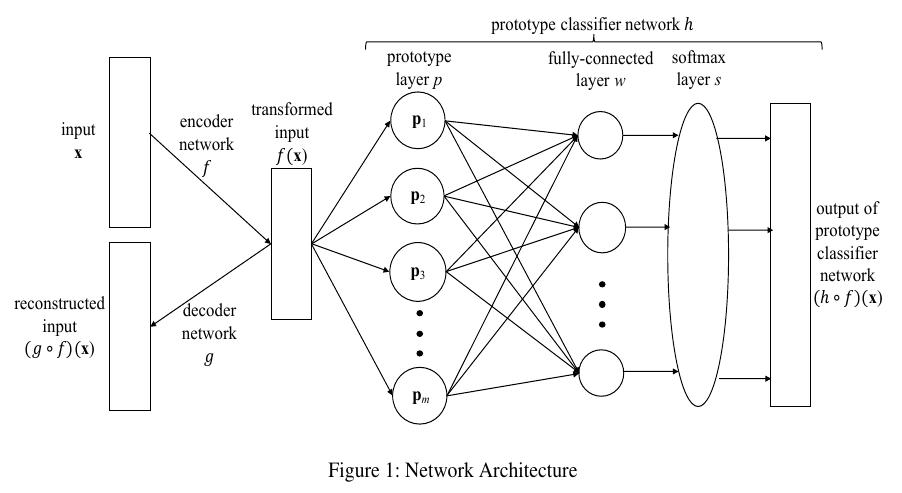
\includegraphics[width=0.5\textwidth]{Images/Li2017.jpg}
    \end{figure}


    \subsection{Explicaciones Generadas}
    \begin{itemize}
        \item \textbf{Prototipos visuales:} Los prototipos se decodifican a imágenes similares a ejemplos reales del conjunto de datos.
        \item \textbf{Interpretación de predicciones:} La clasificación se basa en la cercanía del input codificado a los prototipos más relevantes.
    \end{itemize}

    \subsection{Casos de Estudio}
    \begin{itemize}
        \item \textbf{MNIST:} Precisión del 99.22\%. Los prototipos muestran diferentes estilos de escritura dentro de la misma clase.
        \item \textbf{Cars dataset:} Clasificación de ángulos de visión de autos. Los prototipos eliminan información irrelevante (como el color) y se enfocan en la forma y orientación.
        \item \textbf{Fashion MNIST:} Precisión del 89.95\%. Los prototipos destacan contornos, ignorando detalles como texturas o patrones.
    \end{itemize}

    \subsection{Méritos Adicionales}
    \begin{itemize}
        \item \textbf{Interpretabilidad integrada:} No se necesita análisis posentrenamiento.
        \item \textbf{Regularización:} Los términos de interpretabilidad actúan como regularizadores, reduciendo el sobreajuste.
        \item \textbf{Flexibilidad:} Permite múltiples prototipos por clase, capturando variaciones dentro de las clases.
    \end{itemize}

%%%%%%%%%%%%%%%%%%%%%%%%%%%%%%%%%%%%%%%%%%%%%%%%%%%%%%%%%%%%%%%%%%%%%%%%%%%%%%%

\section{Machine Learning Models to Help Predict Treatment Outcomes in Clinical Gait Analysis}

\subsection{Detalles del Artículo}
\begin{itemize}
    \item \textbf{Título:} Machine Learning Models to Help Predict Treatment Outcomes in Clinical Gait Analysis
    \item \textbf{Autores:} Michael Schwartz, Andrew Ries, Andrew Georgiadis
    \item \textbf{Revista:} Gait \& Posture
    \item \textbf{Nivel:} Publicación en una revista revisada por pares, cuartil Q1 en biomecánica clínica.
    \item \textbf{Fecha de publicación:} Julio de 2024.
\end{itemize}

\subsection{Problema Principal}
El artículo aborda la falta de predictibilidad y la estancada precisión de los resultados de tratamiento guiados por análisis clínico de la marcha. Propone el uso de modelos de aprendizaje automático para generar estimaciones honestas y sin sesgo de los resultados de tratamiento, mejorando así el proceso de toma de decisiones clínicas.

\subsection{Métodos y Diseño del Estudio}
\begin{itemize}
    \item \textbf{Diseño del Estudio:} Análisis retrospectivo utilizando datos de pacientes pediátricos ambulatorios sometidos a diferentes tratamientos de extremidades inferiores.
    \item \textbf{Datos:} Incluye 7450 extremidades tratadas y no tratadas, obtenidas de un centro de análisis de la marcha.
    \item \textbf{Objetivos de Predicción:} Cambios estructurales, funcionales y de actividades relacionados con 12 cirugías comunes (representan más del 95\% de los procedimientos en la base de datos).
    \item \textbf{Método de Evaluación:} Análisis de cobertura honesta y errores absolutos medios (MAE) para evaluar la precisión de los modelos.
\end{itemize}

\subsection{Modelos de Aprendizaje Automático}
\begin{itemize}
    \item \textbf{Algoritmos Utilizados:}
    \begin{itemize}
        \item Direct matching (correspondencia directa): Simple y comprensible para los clínicos.
        \item Modelos estadísticos adicionales para ajuste de sesgos y evaluación de cobertura.
    \end{itemize}
    \item \textbf{Evaluación:} Los modelos fueron evaluados en términos de sesgo, amplitud de intervalos de confianza (CIs) y cobertura promedio:
    \begin{itemize}
        \item \textbf{Cobertura:} 86\% para extremidades tratadas y 87\% para controles.
        \item \textbf{Errores Absolutos Medios (MAE):} Varían según el tipo de predicción y tratamiento.
    \end{itemize}
\end{itemize}

\subsection{Resultados Destacados}
\begin{itemize}
    \item \textbf{Ejemplo 1:} Cambios en el eje bimaleolar después de derotación tibial:
    \begin{itemize}
        \item \textbf{Sesgo:} Inexistente.
        \item \textbf{MAE:} 8º en extremidades tratadas y 6º en controles.
        \item \textbf{Amplitud de CI:} 38º para extremidades tratadas y 27º para controles.
    \end{itemize}
    \item \textbf{Ejemplo 2:} Mejora funcional después de osteotomía femoral:
    \begin{itemize}
        \item Precisión menor en predicciones funcionales debido a datos de entrada menos precisos.
    \end{itemize}
\end{itemize}

\subsection{Discusión y Limitaciones}
\begin{itemize}
    \item \textbf{Fortalezas:}
    \begin{itemize}
        \item Modelos honestos y sin sesgo.
        \item Cobertura consistente y resultados interpretables para los clínicos.
    \end{itemize}
    \item \textbf{Limitaciones:}
    \begin{itemize}
        \item Amplitud subjetivamente amplia de intervalos de confianza.
        \item Necesidad de datos de entrada más precisos (p. ej., mediciones tridimensionales, detalles quirúrgicos cuantitativos).
    \end{itemize}
\end{itemize}

\subsection{Méritos Adicionales}
\begin{itemize}
    \item \textbf{Facilidad de Implementación:} Los modelos son simples y comprensibles para profesionales médicos.
    \item \textbf{Impacto Clínico Potencial:} Integración de predicciones de resultados para mejorar asignaciones de tratamiento basadas en evidencia.
    \item \textbf{Recomendaciones Futuras:} Incorporación de datos avanzados como imágenes 3D y mediciones de fuerza para reducir los intervalos de confianza y mejorar la precisión predictiva.
\end{itemize}


%%%%%%%%%%%%%%%%%%%%%%%%%%%%%%%%%%%%%%%%%%%%%%%%%%%%%%%%%%%%%%%%%%%%%

\section{On the Coherency of Quantitative Evaluation of Visual Explanations}

\subsection{Detalles del Artículo}
\begin{itemize}
    \item \textbf{Título:} On the Coherency of Quantitative Evaluation of Visual Explanations
    \item \textbf{Autores:} Benjamin Vandersmissen, José Oramas
    \item \textbf{Revista:} Computer Vision and Image Understanding (CVIU)
    \item \textbf{Nivel:} Revista revisada por pares, cuartil Q1 en visión por computadora.
    \item \textbf{Fecha de publicación:} Octubre de 2023.
    \item \textbf{DOI:} \href{https://doi.org/10.1016/j.cviu.2024.103934}{10.1016/j.cviu.2024.103934}
\end{itemize}

\subsection{Problema Principal}
El artículo aborda la falta de coherencia en los métodos de evaluación cuantitativa de explicaciones visuales generadas por redes neuronales. Propone un análisis exhaustivo de las métricas más utilizadas para evaluar mapas de calor de saliencia en modelos aplicados a tareas de visión por computadora.

\subsection{Arquitectura del Modelo y Métodos}
\begin{itemize}
    \item Se analizaron los modelos \textbf{ResNet-50} y \textbf{VGG16}, entrenados con pesos preentrenados en ImageNet.
    \item Métodos de explicación visual evaluados:
    \begin{itemize}
        \item Métodos basados en gradiente: SmoothGrad, Grad-CAM, Integrated Gradients (IG).
        \item Métodos de retropropagación: Layer-wise Relevance Propagation (LRP).
        \item Métodos basados en perturbación: Occlusion, RISE.
        \item Otros: AdaSISE, TAME.
    \end{itemize}
\end{itemize}

\subsection{Métricas de Evaluación}
\begin{itemize}
    \item \textbf{Insertion y Deletion Curves:}
    \begin{itemize}
        \item AUC para insertar píxeles relevantes: AdaSISE y RISE lideran con 0.642.
        \item AUC para eliminar píxeles relevantes: TAME logra 0.176.
    \end{itemize}
    \item \textbf{Average Drop (\%):} Métrica para evaluar cómo el puntaje del modelo cambia al usar solo las regiones destacadas:
    \begin{itemize}
        \item Mejores resultados: RISE (14.02\%), Grad-CAM (14.96\%).
    \end{itemize}
    \item \textbf{Pointing Game:} Evalúa la localización de los objetos relevantes:
    \begin{itemize}
        \item Mayor precisión: AdaSISE (92.77\%).
    \end{itemize}
\end{itemize}

\subsection{Conclusiones Clave}
\begin{itemize}
    \item \textbf{Inconsistencias entre métricas:} Métricas como Insertion y Deletion reflejan nociones opuestas de "bondad" en las explicaciones.
    \item \textbf{Impacto de la Sparsidad:} Mapas de calor más densos favorecen métricas como Insertion, mientras que mapas dispersos benefician métricas como Deletion.
    \item \textbf{Recomendaciones:} Se desaconseja el uso de métricas basadas en tareas proxy, como el Pointing Game, debido a su baja correlación con otras métricas.
\end{itemize}

\end{document}
